\documentclass[11pt]{article}
\usepackage[margin=1in]{geometry}
\usepackage{amsmath,amssymb}
\usepackage{graphicx}
\usepackage{booktabs}
\usepackage{array}
\usepackage{xcolor}
\usepackage[colorlinks=true,linkcolor=blue,urlcolor=blue]{hyperref}
\usepackage{siunitx}

% tier colors matching the plot
\definecolor{tierGrey}{rgb}{0.55,0.55,0.60}
\definecolor{tierLight}{rgb}{0.35,0.60,0.30}
\definecolor{tierDark}{rgb}{0.10,0.45,0.15}

\newcommand{\dV}{\Delta V}
\newcommand{\tf}{t_f}
\newcommand{\lamv}{\boldsymbol{\lambda}_v}
\newcommand{\lamm}{\lambda_m}

\title{The Honest $\dV$--$\tf$ Front for the Min-Fuel GTO$\to$Tulip Transfer\\
\large Reading \texttt{front\_honest.png}, and the first-switch anomaly}
\author{Min-fuel campaign notes, \texttt{sundman\_minfuel/}}
\date{2026-07-09}

\begin{document}
\maketitle

\begin{abstract}
\noindent
This note explains the figure \texttt{results/plots/front\_honest.png}: what is
plotted, what every color and line means, and how each point is certified. It
then treats in detail the one open blemish on the front --- the \emph{first-switch
anomaly} --- which is the reason two shades of green exist rather than one.
\end{abstract}

\section{What is plotted}

We solve the minimum-fuel low-thrust transfer from GTO to a tulip orbit in the
Earth--Moon circular restricted three-body problem (CR3BP). The spacecraft is
\SI{15}{kg}, thrusts at \SI{25}{mN}, with $I_{sp}=\SI{2100}{s}$; the transfer is
a $\sim$40-revolution spiral. In each optimization the transfer time $\tf$ is
\textbf{fixed}, and we minimize propellant, equivalently
$\dV = c\,\ln(m_0/m_f)$ with $c=I_{sp}g_0$ the exhaust speed. Solving
independently at many $\tf$ and plotting $\dV(\tf)$ traces the fuel--time trade.

The reference point is the minimum-\emph{time} solution: $\tf^{\min}=
6.2906939607$ ND $=\SI{27.8845}{d}$, which burns continuously (zero coasts) and
costs $\dV=\SI{4.4665}{km/s}$. Every fixed-time point is labeled by its
\emph{factor} $\tf/\tf^{\min}$ (1.12$\times$, 1.65$\times$, \dots), though the
plot's horizontal axis is in days.

Each solve is a Sundman-regularized trapezoidal collocation NLP (CasADi +
IPOPT), reached by a Bertrand--\'Ep\'enoy energy-to-fuel homotopy. \textbf{Every
plotted point is feasible to machine precision} --- dynamics defects
$\sim\!10^{-14}$, boundary conditions exact. Feasibility is never the question.
What differs point to point is \emph{how strongly we can certify optimality},
and that is what the colors encode.

\section{The honesty problem this plot solves}

A direct NLP returns only a \emph{local} minimum, and this landscape has many:
distinct solution families with different coast/burn switch counts, connected
over a fold near $1.40$--$1.45\times$. A naive ``one solution per $\tf$'' plot
would hide two failure modes:
\begin{enumerate}
\item A converged point can be a \emph{worse} local minimum than another
solution we already hold at the same $\tf$ (a dominated point masquerading as
the front).
\item A converged point may fail the first-order Pontryagin necessary
conditions when checked against its own KKT duals --- feasible, but not
demonstrably an extremal.
\end{enumerate}
The policy, therefore: plot \emph{every} stored solution, color each by how much
verification it survives, and draw two envelopes that separate ``certified''
from merely ``best known.''

\section{How each point is certified (empirical-$\beta$)}
\label{sec:cert}

For the min-fuel problem the throttle $s\in[0,1]$ enters the Hamiltonian
linearly, so Pontryagin's principle makes it \emph{bang--bang}, switching on the
sign of a switching function. With the discrete costates recovered from the
NLP's own constraint duals ($\texttt{lamDef}$, the $8\times N$ KKT multipliers on
the dynamics defects), the switching function is
\begin{equation}
  S \;=\; 1 - \beta\,W,
  \qquad
  W \;=\; \frac{\lVert\lamv\rVert\,c}{m} - \lamm ,
  \label{eq:S}
\end{equation}
where $\lamv$ is the primer (velocity costate), $\lamm$ the mass costate, and
$\beta>0$ a single positive scale that absorbs the trapezoid-weight / Sundman
time-dilation normalization of the discrete covector. The optimal control burns
($s=1$) where $S<0$ and coasts ($s=0$) where $S>0$ (the global sign of $W$ was
fixed empirically and verified). The thrust direction is anti-parallel to the
primer, $\hat{\boldsymbol{\alpha}}=-\lamv/\lVert\lamv\rVert$.

The key idea: at every throttle \emph{switch} the control changes, so $S$ must
vanish there. Equation~\eqref{eq:S} then \emph{implies} a scale at switch $k$,
\begin{equation}
  \beta_k \;=\; 1/W_k .
\end{equation}
If the trajectory is a true extremal, all $\beta_k$ must agree --- the switches
\emph{over-determine} $\beta$, and their mutual agreement is the test. We take
\begin{equation}
  \beta \;=\; \operatorname{median}_k\,\beta_k
\end{equation}
(robust; an earlier least-squares $\beta$ was dragged by a single outlier switch
and produced cascading false failures, diagnosed by \texttt{diag\_beta\_checker.m}).

\paragraph{Gates.} A point passes the interior certification when, with this
robust $\beta$:
\begin{itemize}
\item $\operatorname{sign}(S)$ is correct on $\ge 99\%$ of burn intervals
\emph{and} $\ge 99\%$ of coast intervals;
\item the robust spread of the $\beta_k$ (median absolute deviation) is
$\le 5\%$;
\item the thrust direction aligns with the primer to $\le 0.2^\circ$;
\item transversality holds: $|\lamm(\tf)| \le 10^{-3}\max_k|\lamm|$
(relative, hence scale-invariant).
\end{itemize}

\paragraph{Two tiers.} All gates pass \emph{and} the first switch is consistent,
$|\beta_1/\beta - 1|\le 0.10$ $\Rightarrow$ \textbf{FULL} certification. All
gates pass but the first switch is off by more than $10\%$ $\Rightarrow$
\textbf{interior} certification (the first-switch question is flagged, not
hidden). Any gate fails $\Rightarrow$ \textbf{feasible only}.

\section{Reading the figure}

\begin{figure}[h]
\centering
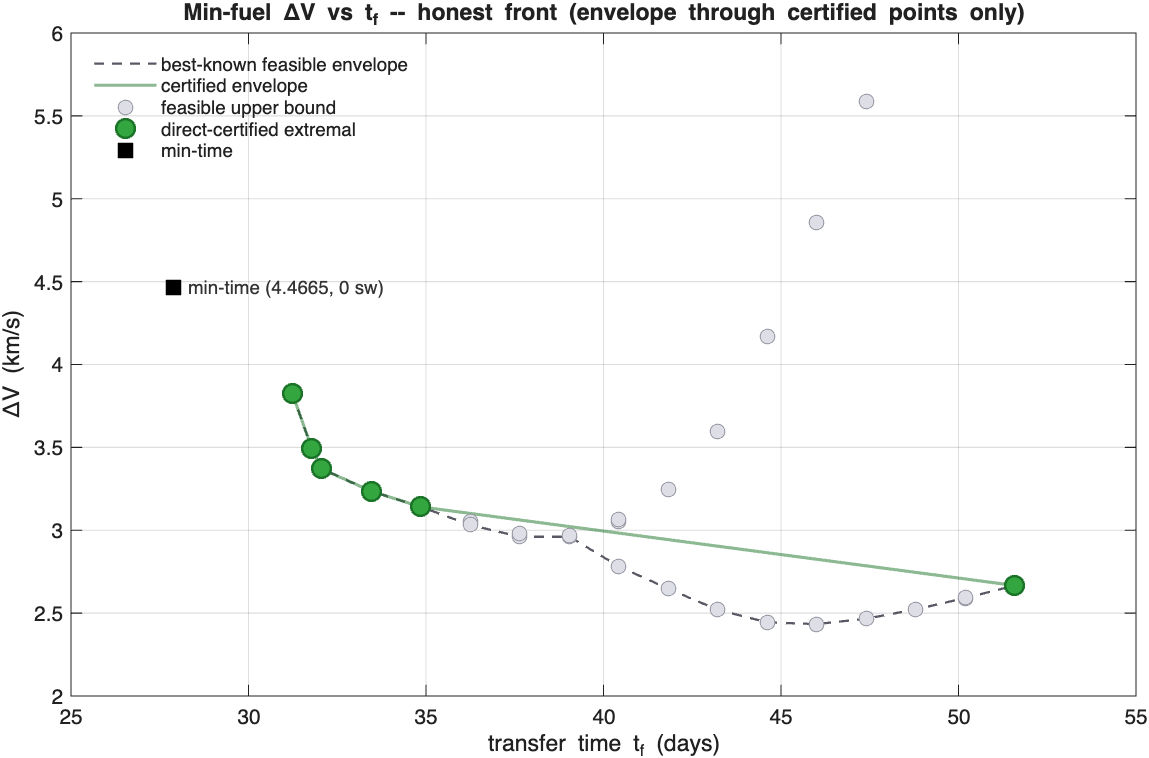
\includegraphics[width=\textwidth]{results/plots/front_honest.png}
\caption{The honest $\dV$--$\tf$ front. Every marker is a machine-feasible
stored solution; color is its certification tier. Solid line: certified
envelope. Dashed line: best-known feasible envelope. Black square: min-time
anchor. As of this writing the two envelopes coincide everywhere.}
\label{fig:front}
\end{figure}

\paragraph{Markers (Fig.~\ref{fig:front}).} Each circle is one stored solution;
several may share a $\tf$ (different seeds/branches). The color is its tier from
Section~\ref{sec:cert}:
\begin{center}
\renewcommand{\arraystretch}{1.3}
\begin{tabular}{>{\raggedright}p{3.1cm} p{2.4cm} p{8.2cm}}
\toprule
\textbf{Marker} & \textbf{Class} & \textbf{Meaning} \\
\midrule
{\color{tierGrey}$\bullet$}~grey &
feasible upper bound &
Dynamics + BCs machine-tight, but a PMP gate \emph{failed}. A rigorous upper
bound: the true optimum here is at or below it. (3 points --- older scatter with
genuine coast-sign inconsistencies.) \\
{\color{tierLight}$\bullet$}~light green &
interior-certified &
All PMP gates pass with robust $\beta$, \emph{except} the first switch
(Section~\ref{sec:firstswitch}). Certified extremal on the trajectory interior,
one flagged open question. (25 points --- the whole envelope $1.25$--$1.80\times$,
including the minimum.) \\
{\color{tierDark}$\bullet$}~dark green &
FULL certified &
Everything above, and the first switch is consistent too. No direct-method
caveat. (6 points: 1.12, 1.14, 1.15, 1.20, 1.85, plus a 1.85 duplicate.) \\
$\blacksquare$~blue &
direct+indirect &
Reserved for agreement with an independent indirect (shooting) solution. None
yet --- the class is empty by design until the \texttt{ms\_band} arbiter runs. \\
\bottomrule
\end{tabular}
\end{center}

\paragraph{The two envelope lines.} These are the pair most worth getting right:
\begin{itemize}
\item \textbf{Solid green --- certified envelope.} Through the best
\emph{certified} point (class $\ge$ light green) at each $\tf$. This is the curve
we will \emph{defend as first-order extremal}.
\item \textbf{Dashed grey --- best-known feasible envelope.} Through the minimum
$\dV$ over \emph{all} points at each $\tf$, certified or not. Because every point
is feasible, this is the honest statement ``the true front lies at or below
here.''
\end{itemize}
\textbf{Reading rule:} wherever the dashed line dips \emph{below} the solid one,
an uncertified solution beats the best certified one --- a flag that a better
local minimum is hiding and the certification needs work. As of 2026-07-09
\textbf{the two lines coincide everywhere}: at every $\tf$ the best-known
solution is also a certified one. That coincidence is the figure's headline.

\paragraph{Stacked markers --- two certified circles at the same $\tf$.} You will
see light-green circles sitting \emph{directly above} other light-green circles
at the same transfer time (clearest near $1.45$--$1.55\times$; e.g.\ at
$1.55\times$ one interior point at $\dV=\SI{2.52}{km/s}$ with 31 switches and
another at $\dV=\SI{3.60}{km/s}$ with 45 switches). This is not a plotting glitch
--- it is the whole reason for the honest-plot policy. At a fixed $\tf$ the
min-fuel problem has \emph{several coexisting local minima}: distinct solution
families with different burn/coast switch counts, reached from different seeds
(the energy backbone, the neighbor chains, the down-chain). Each converges to its
\emph{own} feasible extremal, and \emph{each can independently pass the interior
PMP gates} --- so both earn a green marker. They simply cost different amounts of
fuel.

The lower circle is the better local minimum at that $\tf$; the higher one is a
genuinely first-order-optimal solution of a \emph{different} family that happens
to be more expensive --- a \emph{dominated extremal}. The certified envelope
(solid green) takes the minimum over certified points, so it rides the lower
circles and the upper ones sit visibly above it. We keep those upper markers on
the plot on purpose: they are the visual proof that ``certified'' means
\emph{first-order optimal within its family}, \emph{not} globally best --- a
certified point can still be beaten by another certified point at the same
$\tf$. (When two stacked circles have essentially the \emph{same} $\dV$ --- e.g.\
the two coincident points at $1.85\times$ or $1.75\times$ --- they are instead
the same solution recovered by two different seeds/branches, a reproducibility
check rather than a distinct family.)

\paragraph{The black square} at $(\SI{27.88}{d},\,\SI{4.4665}{km/s})$ is the
min-time anchor: zero coasts, maximum $\dV$. Every min-fuel point lies to its
right (more time) and below it (less $\dV$).

\paragraph{Shape of the front.} $\dV$ falls steeply as $\tf$ grows --- extra time
buys efficient coast arcs through apogee. The campaign minimum is
$\dV=\SI{2.434}{km/s}$ at $1.65\times$ ($\approx\SI{46}{d}$), $45.5\%$ below
min-time. Past $1.65\times$ the stored values \emph{rise} again, but those points
are \emph{dominated}: by loiter monotonicity (any solution at $\tf$ can be flown
at $\tf'>\tf$ by appending terminal coast), the true front for $\tf\ge1.65\times$
is $\le\SI{2.434}{km/s}$. So the $1.70$--$1.85\times$ certified points are honest
extremals \emph{of their family} yet known not to be on the front there ---
``certified'' and ``on the true front'' are different claims, and the plot keeps
them separate. The band $1.01$--$1.11\times$, just above min-time, is absent: a
hard bifurcation zone that resists direct methods so far (a separate
multiple-shooting attack is underway there).

\section{The first-switch anomaly}
\label{sec:firstswitch}

This is the one blemish that keeps most of the front at ``interior'' rather than
``FULL,'' so it deserves detail.

\subsection{The observation}

Run the empirical-$\beta$ check and look at the implied per-switch scales
$\beta_k=1/W_k$ individually. On \emph{every} solution across the band, all
switches \emph{except the very first} agree with each other superbly --- their
spread (MAD) is under $0.8\%$, essentially a flat line at a common value. The
\emph{first} switch is the lone exception: its implied scale
$\beta_1/\beta$ departs from 1, and it does so \emph{smoothly and
systematically} as $\tf$ grows. Table~\ref{tab:firstsw} shows the best-certified
solution at each factor.

\begin{table}[h]
\centering
\caption{Best-certified solution per factor. $\beta_1/\beta$ is the first-switch
implied scale relative to the robust common scale; MAD is the robust spread over
\emph{all} switches. Every row passes the interior gates (burn/coast signs
$100\%$/$\ge99.8\%$, MAD $\ll5\%$). ``FULL'' requires $|\beta_1/\beta-1|\le0.10$.}
\label{tab:firstsw}
\renewcommand{\arraystretch}{1.15}
\sisetup{table-format=1.3}
\begin{tabular}{S[table-format=1.2] S[table-format=2.2] S[table-format=1.4] S[table-format=2.0] S[table-format=1.3] S[table-format=1.3] l}
\toprule
{factor} & {days} & {$\dV$ (km/s)} & {switches} & {$\beta_1/\beta$} & {MAD (\%)} & {tier} \\
\midrule
1.12 & 31.23 & 3.8278 & 12 & 0.995 & 0.135 & {\color{tierDark}FULL} \\
1.14 & 31.79 & 3.4905 & 26 & 0.996 & 0.351 & {\color{tierDark}FULL} \\
1.15 & 32.07 & 3.3696 & 24 & 1.003 & 0.261 & {\color{tierDark}FULL} \\
1.20 & 33.46 & 3.2355 & 44 & 0.931 & 0.159 & {\color{tierDark}FULL} \\
1.25 & 34.86 & 3.1409 & 50 & 0.838 & 0.158 & {\color{tierLight}interior} \\
1.30 & 36.25 & 3.0318 & 42 & 0.687 & 0.204 & {\color{tierLight}interior} \\
1.35 & 37.64 & 2.9606 & 30 & 0.505 & 0.188 & {\color{tierLight}interior} \\
1.40 & 39.04 & 2.9609 & 26 & 0.317 & 0.288 & {\color{tierLight}interior} \\
1.45 & 40.43 & 2.7818 & 43 & 0.123 & 0.787 & {\color{tierLight}interior} \\
1.50 & 41.83 & 2.6469 & 35 & 0.129 & 0.731 & {\color{tierLight}interior} \\
1.55 & 43.22 & 2.5198 & 31 & 0.149 & 0.510 & {\color{tierLight}interior} \\
1.60 & 44.62 & 2.4441 & 27 & 0.189 & 0.446 & {\color{tierLight}interior} \\
1.65 & 46.01 & 2.4339 & 23 & 0.232 & 0.401 & {\color{tierLight}interior} \\
1.70 & 47.40 & 2.4664 & 23 & 0.254 & 0.492 & {\color{tierLight}interior} \\
1.75 & 48.80 & 2.5227 & 23 & 0.258 & 0.303 & {\color{tierLight}interior} \\
1.80 & 50.19 & 2.5911 & 23 & 0.271 & 0.278 & {\color{tierLight}interior} \\
1.85 & 51.59 & 2.6667 & 22 & 0.996 & 0.338 & {\color{tierDark}FULL} \\
\bottomrule
\end{tabular}
\end{table}

Figure~\ref{fig:beta} makes it visual: the right-hand panels plot $\beta_k$ per
switch index. The bulk sits dead flat at 1; the first index is the single
outlier, and its offset grows with $\tf$.

\begin{figure}[h]
\centering
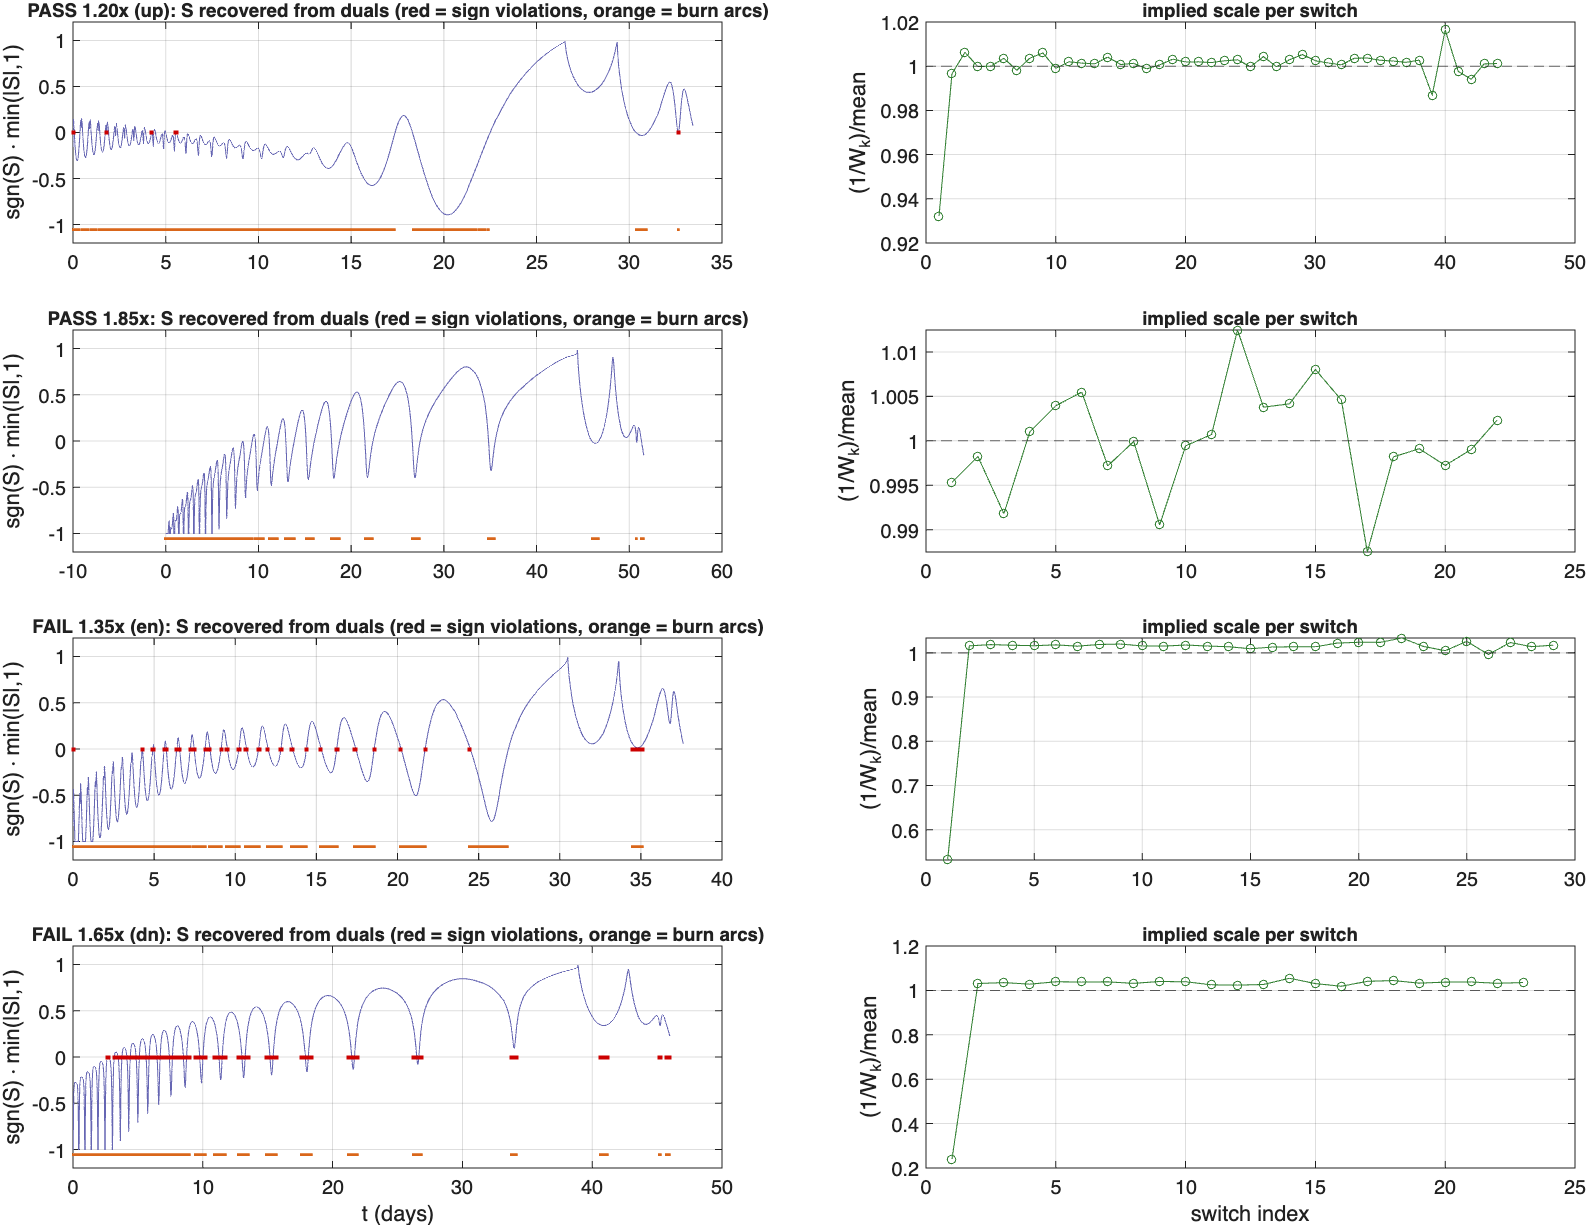
\includegraphics[width=\textwidth]{results/plots/beta_checker_diag.png}
\caption{Diagnostic from \texttt{diag\_beta\_checker.m} on four representative
cases. Left panels: the switching function $S$ recovered from the duals (orange
= burn arcs, red = sign violations) --- violations, where present, sit right
\emph{at} switch crossings, not filling whole arcs. Right panels: the implied
per-switch scale $\beta_k/\overline{\beta_k}$ versus switch index --- a flat line
at 1 except for the first index, which is the anomaly.}
\label{fig:beta}
\end{figure}

\subsection{Reading the diagnostic figure in full}
\label{sec:diag}

Figure~\ref{fig:beta} is the output of \texttt{diag\_beta\_checker.m}, a
purpose-built tool that answers \emph{why} the na\"ive check failed on the upper
band while passing at the anchors. It operates entirely on saved KKT duals (no
re-solving) and was written to discriminate three competing explanations for a
failing switching-law check:
\begin{description}
\item[H1 --- gate artifact.] Sign violations live only in the $\pm1$-interval
window \emph{around} switches, where the trapezoid midpoint straddles $S=0$ and
the sign is genuinely ambiguous at mesh resolution. Signature: violation mass
concentrated at distance $\le1$ from a switch.
\item[H2 --- wrong switch pattern.] Violations fill \emph{whole arcs} --- an arc
that should coast burns, or vice versa. The switch structure is not
extremal-supported. Signature: some arcs $>50\%$ violating (``flipped'' arcs).
\item[H3 --- scale drift.] The single-$\beta$ model itself breaks: the implied
$\beta_k$ \emph{drifts} systematically along the trajectory instead of scattering
about a constant. Signature: a strong monotone correlation of $\beta_k$ with
switch index / time.
\end{description}

The figure runs four representative cases, chosen to span pass and fail: a
passing up-backbone point ($1.20\times$), the clean anchor ($1.85\times$), and
two that failed the \emph{old} least-squares gate ($1.35\times$ from the energy
chain, $1.65\times$ from the down-chain). Each row is one case, with two panels:

\begin{itemize}
\item \textbf{Left panel --- the switching function from the duals.} The blue
trace is $\operatorname{sgn}(S)\cdot\min(|S|,1)$ recovered from
Eq.~\eqref{eq:S} along the trajectory; orange dots mark the burn arcs; red dots
mark any sign violations. The takeaway across all four cases: the red dots, where
they appear, sit \emph{at} the switch crossings, not spread through the arc
interiors. That is the H1 signature and rules out H2 --- the burn/coast
\emph{pattern} is right; only the razor's-edge sign at the crossing is
ambiguous.
\item \textbf{Right panel --- the implied scale per switch.} This plots
$\beta_k/\overline{\beta_k}$ against switch index with a dashed reference line at
1. In every case the points lie flat on 1 --- \emph{except} the first index.
There is no monotone ramp across the indices, which rules out H3 (no global scale
drift): the single-$\beta$ model is sound; one switch is simply off.
\end{itemize}

\noindent The diagnostic's verdict, then, was decisive and is what motivated the
present gate: the upper-band ``failures'' were \emph{not} H2 (bad structure) or
H3 (model breakdown), but an H1-flavored effect localized to the \emph{first}
switch, amplified into a whole-front failure only because the old least-squares
$\beta$ let that one outlier drag the fit. Replacing least-squares with the
robust median $\beta$ (Section~\ref{sec:cert}) and isolating the first switch into
its own tier is the direct consequence of these four panels.

\subsection{Why it forces the two-tier gate}

Because the anomaly is confined to \emph{one} switch out of dozens, it does not
corrupt the robust median $\beta$ or the MAD gate (Table~\ref{tab:firstsw}: MAD
stays well under $1\%$ even when $\beta_1/\beta$ has fallen to $0.12$). The
robust estimator was specifically chosen so this single outlier cannot poison
the whole certification --- which is why the entire interior of every trajectory
still certifies. The two-tier gate then \emph{quarantines} exactly this one
question: FULL if the first switch also matches, interior if it is the lone
holdout. Nothing is swept under the rug; the offset is measured and reported per
point. (Concretely, $1.25\times$ was \emph{demoted} from the old certified set by
this analysis --- $\beta_1/\beta=0.838$ --- an example of the gate being honest
rather than generous.)

\subsection{What it could be --- two hypotheses}

The offset is real and systematic, not numerical noise. Two explanations remain
open:
\begin{description}
\item[H1: mesh under-resolution at the first switch.] The first switch happens
early in the transfer, deep in the gravity well where the dynamics are fastest
even after Sundman regularization. If the collocation mesh is locally too coarse
there, the discrete costate at that switch is inaccurate, biasing $\beta_1$
without affecting the well-resolved later switches. This is a
\emph{discretization} artifact --- the continuous extremal is fine; our
recovered dual at one node is not.
\item[H2: genuine local non-extremality of the first arc.] The first burn/coast
boundary is genuinely not where a true extremal would place it --- the direct
solver has found a nearby feasible point that is not first-order optimal in that
one structural feature.
\end{description}

\subsection{The evidence leans toward H1}

Two data patterns point at the mesh/continuation explanation, though neither is
decisive:

\begin{enumerate}
\item \textbf{The clean points are the independently solved ones.} The only
rows with $\beta_1/\beta\approx1$ are the two \emph{anchors} solved fresh, not by
continuation: the low band $1.12$--$1.15\times$ (built directly from the energy
backbone) and $1.85\times$ (the original certified result). \emph{Every} point
reached by continuation away from an anchor shows the anomaly, and it deepens
monotonically \emph{with distance from the anchor} --- from $1.20\times$
($0.931$) walking up, and from $1.80\times$ ($0.271$) walking down from the clean
$1.85\times$ ($0.996$). An intrinsic non-extremality (H2) would not care which
$\tf$ we happened to solve independently; a continuation/mesh artifact would.
\item \textbf{The violations are at the switches, not in the arcs.} The
diagnostic (Fig.~\ref{fig:beta}, left panels, and the ``near-switch'' statistic
in \texttt{diag\_beta\_checker.m}) shows what sign violations exist cluster in
the $\pm1$-interval window \emph{around} switch crossings --- where the
trapezoid midpoint straddles $S=0$ and the sign is ambiguous at mesh resolution
--- rather than filling whole arcs (which would be the signature of a genuinely
mis-placed burn/coast structure, H2).
\end{enumerate}

\subsection{How it will be settled}

The definitive arbiter is an \emph{independent indirect} solve of the same
transfer via the multiple-shooting machinery (\texttt{ms\_band}), currently being
proven on the lower band. An indirect method carries the \emph{exact continuous}
costates, with no discrete-dual recovery and no collocation mesh. If its first
switch lands where the direct solution puts it, the direct answer is vindicated
and the anomaly is confirmed as our dual-recovery artifact (H1); if not, H2
stands and the first arc genuinely needs re-solving. Either outcome promotes the
affected points to the (currently empty) blue direct+indirect class. Until then,
the honest statement is exactly what the plot shows: interior-certified, first
switch flagged.

\section{What the plot does and does not claim}

\begin{itemize}
\item \textbf{Not} global optimality. Green means the solution satisfies the
first-order necessary conditions per its own duals; a better family could exist
at any $\tf$. The dashed line is only ``best known.''
\item \textbf{No} second-order / conjugate-point test anywhere yet.
\item \textbf{No} independent-method confirmation yet (blue class empty).
\item Light-green points carry the explicit first-switch caveat above.
\item The $1.70$--$1.85\times$ certified points are extremals of their family and
simultaneously known to be dominated --- two different claims, kept separate.
\end{itemize}

\paragraph{Regenerate.} Run \texttt{aggregate\_front} in MATLAB from
\texttt{sundman\_minfuel/}; it re-verifies every stored solution and rewrites
\texttt{results/plots/front\_honest.png}. Companion documents:
\begin{itemize}
\item \texttt{FRONT\_HONEST\_PLOT\_EXPLAINED.md} --- Markdown twin of this note;
\item \texttt{HONEST\_EVALUATION\_DV\_TF\_FRONT.md} --- policy and candid assessment;
\item \texttt{LOW\_THRUST\_MINFUEL\_CAMPAIGN.md} --- full campaign log.
\end{itemize}

\end{document}
